%% ============================================================
%%  Chapter 10 — Planning & Schedule Management
%%  Project Planning & Prototyping (247-519-VA), Vanier College
%% ============================================================

\chapter{Planning \& Schedule Management}
\label{ch:planning}

\paragraph{Where this fits.}
This chapter is a \textbf{Stage~3 (Development)} deliverable.
A realistic project schedule and an updated risk register are
\textbf{Gate~3} artefacts; a schedule built on optimistic guesses or
missing lead times is a gate failure \emph{before} the prototype is
assembled.

Chapter~9 established the electrical and safety architecture of the
IoT robotic sorting subsystem: the power budget confirmed a 50.5-day
battery life at $I_{\text{avg}} = 1.649\ \text{mA}$, and the safety
design log recorded a load-path safety factor of $SF = 5.29$.
That work left one critical question unanswered: \emph{in what order
does the team build everything, and when will it be done?}
This chapter answers that question.
You will decompose the build into a Work Breakdown Structure, link
activities with dependencies, identify the critical path, handle
procurement lead times as explicit schedule risks, and finish with a
Gantt chart and an updated risk register.

\paragraph{Learning Objectives.}
By the end of this chapter you will be able to:
\begin{enumerate}
  \item Identify all project activities, organise them into a
        \textbf{Work Breakdown Structure} (WBS), and determine the
        critical path using the Critical Path Method (CPM).
  \item \textbf{Build} a Gantt chart from CPM results, annotating critical-path bars, slack extensions on non-critical activities, and milestone markers.
  \item Compute early/late start and finish times, slack, and the
        critical path for a multi-activity network.
  \item Estimate activity durations under uncertainty by applying the
        PERT three-point formula and interpreting the resulting
        standard deviation.
  \item Maintain a living risk register that treats procurement lead
        times and supplier delays as first-class schedule risks.
\end{enumerate}

% ============================================================
\section{Work Breakdown Structure}
\label{sec:wbs}
% ============================================================

A \textbf{Work Breakdown Structure}\index{Work Breakdown Structure}
(WBS) is a hierarchical decomposition of all the work required to
complete the project.
Every leaf node of the WBS is a \textbf{work package}\index{work package}:
a discrete, assignable, and estimable unit of effort.

\subsection{Why decompose first?}

Dependencies, durations, and risks can only be managed once work is
visible.
A single task labelled ``build the prototype'' cannot be scheduled,
assigned, or monitored.
Breaking it into atomic work packages — PCB design, component
procurement, firmware integration, system test — makes each element
plannable and observable.

\subsection{WBS for the sorter prototype}

The sorter build decomposes into two top-level branches: \emph{Hardware}
and \emph{Software}.
Under Hardware the packages are PCB design (A), component procurement
(B), PCB fabrication (C), and PCB assembly (D).
Under Software the packages are firmware integration (E).
System test (F) spans both branches and sits at the integration level.

\begin{table}[h]
  \centering
  \caption{WBS work packages for the sorter prototype build.}
  \label{tab:wbs}
  \begin{tabular}{clcl}
    \hline
    \textbf{ID} & \textbf{Work package} & \textbf{Duration (d)} &
    \textbf{Predecessors} \\
    \hline
    A & PCB design           & 3 & --- \\
    B & Component procurement & 7 & A   \\
    C & PCB fabrication      & 5 & A   \\
    D & PCB assembly         & 2 & B, C \\
    E & Firmware integration & 4 & A   \\
    F & System test          & 3 & D, E \\
    \hline
  \end{tabular}
\end{table}

\paragraph{In Practice.}
WBS depth should match the team's ability to estimate and track.
For a four-week prototype sprint, work packages of one to five days are
practical; packages longer than a week are usually hiding sub-tasks that
carry independent risks.

% ============================================================
\section{Dependencies and Critical Path}
\label{sec:cpm}
% ============================================================

\subsection{Activity-on-node notation}

In the \textbf{Critical Path Method}\index{Critical Path Method} (CPM)
each work package is drawn as a node and each dependency as a directed
arc from predecessor to successor.
Figure~\ref{fig:cpm_network} shows the six-activity network for the
sorter build; the critical path is highlighted with bold arcs.

\begin{figure}[h]
  \centering
  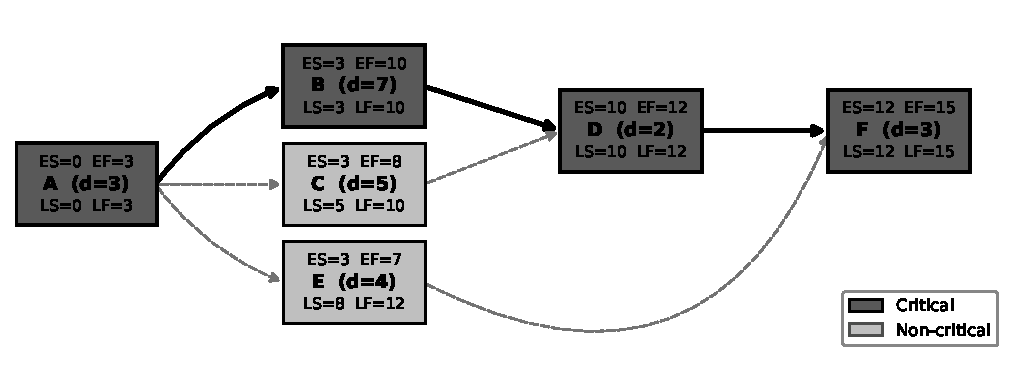
\includegraphics[width=0.85\textwidth]{images/fig_02_cpm_network}
  \caption{Activity-on-node CPM network for the sorter prototype build.
           Bold arcs mark the critical path A\,$\to$\,B\,$\to$\,D\,$\to$\,F
           (15 days). Numbers inside each node show ES\,/\,EF on the top row
           and LS\,/\,LF on the bottom row.}
  \label{fig:cpm_network}
\end{figure}

\subsection{Forward pass — earliest start and finish}

The \textbf{early start}\index{early start} (ES) of an activity is the
earliest day on which it can begin, given all predecessors are complete.
The \textbf{early finish}\index{early finish} (EF) is:
$EF = ES + \text{duration}$.

Processing the network from left to right:

\begin{enumerate}
  \item[(A)] $ES_A = 0$; \quad $EF_A = 0 + 3 = 3$
  \item[(B)] $ES_B = EF_A = 3$; \quad $EF_B = 3 + 7 = 10$
  \item[(C)] $ES_C = EF_A = 3$; \quad $EF_C = 3 + 5 = 8$
  \item[(D)] $ES_D = \max(EF_B,\, EF_C) = \max(10,\, 8) = 10$; \quad
             $EF_D = 10 + 2 = 12$
  \item[(E)] $ES_E = EF_A = 3$; \quad $EF_E = 3 + 4 = 7$
  \item[(F)] $ES_F = \max(EF_D,\, EF_E) = \max(12,\, 7) = 12$; \quad
             $EF_F = 12 + 3 = 15$
\end{enumerate}

The \textbf{project duration}\index{project duration} is
$T = EF_F = \mathbf{15\ \text{days}}$.

\subsection{Backward pass — latest start and finish}

The \textbf{late finish}\index{late finish} (LF) of an activity is the
latest day by which it must finish without delaying the project.
The \textbf{late start}\index{late start} (LS) is:
$LS = LF - \text{duration}$.

Processing right to left (setting $LF_F = 15$):

\begin{enumerate}
  \item[(F)] $LF_F = 15$; \quad $LS_F = 15 - 3 = 12$
  \item[(D)] $LF_D = LS_F = 12$; \quad $LS_D = 12 - 2 = 10$
  \item[(E)] $LF_E = LS_F = 12$; \quad $LS_E = 12 - 4 = 8$
  \item[(C)] $LF_C = LS_D = 10$; \quad $LS_C = 10 - 5 = 5$
  \item[(B)] $LF_B = LS_D = 10$; \quad $LS_B = 10 - 7 = 3$
  \item[(A)] $LF_A = \min(LS_B,\, LS_C,\, LS_E) = \min(3,\, 5,\, 8) = 3$;
             \quad $LS_A = 3 - 3 = 0$
\end{enumerate}

\subsection{Slack and the critical path}

\textbf{Slack}\index{slack} (also called float) is the amount by which
an activity can be delayed without extending the project:

\begin{equation}
  \text{slack} = LS - ES = LF - EF
  \label{eq:ch10-slack}
\end{equation}

Applying Equation~\ref{eq:ch10-slack} to each activity:

\begin{table}[h]
  \centering
  \caption{CPM results for the sorter prototype build.}
  \label{tab:cpm}
  \begin{tabular}{clccccccc}
    \hline
    \textbf{ID} & \textbf{Package} & \textbf{Dur} &
    \textbf{ES} & \textbf{EF} & \textbf{LS} & \textbf{LF} &
    \textbf{Slack} & \textbf{Critical?} \\
    \hline
    A & PCB design           & 3 &  0 &  3 &  0 &  3 & 0 & \textbf{Yes} \\
    B & Component procurement & 7 &  3 & 10 &  3 & 10 & 0 & \textbf{Yes} \\
    C & PCB fabrication      & 5 &  3 &  8 &  5 & 10 & 2 & No           \\
    D & PCB assembly         & 2 & 10 & 12 & 10 & 12 & 0 & \textbf{Yes} \\
    E & Firmware integration & 4 &  3 &  7 &  8 & 12 & 5 & No           \\
    F & System test          & 3 & 12 & 15 & 12 & 15 & 0 & \textbf{Yes} \\
    \hline
  \end{tabular}
\end{table}

The \textbf{critical path}\index{critical path} consists of every
activity with zero slack.
Here that is \textbf{A\,$\to$\,B\,$\to$\,D\,$\to$\,F}, with a total
duration of $3 + 7 + 2 + 3 = \mathbf{15\ \text{days}}$.

The competing path A\,$\to$\,C\,$\to$\,D\,$\to$\,F spans only
$3 + 5 + 2 + 3 = 13$~days, giving C a slack of~2~days.
Path A\,$\to$\,E\,$\to$\,F spans $3 + 4 + 3 = 10$~days, giving E a
slack of~5~days.

\paragraph{Common Pitfalls.}
A common error is to identify the critical path as the sequence
containing the \emph{longest single task}.
Activity B (7~days) is the longest task, but the critical path is
defined by \emph{total path length}, not individual activity duration.
A short activity with zero slack (e.g., PCB assembly at 2~days) is just
as critical as the longest one.

% ============================================================
\section{Gantt Scheduling}
\label{sec:gantt}
% ============================================================

A \textbf{Gantt chart}\index{Gantt chart} maps each work package to a
horizontal bar on a calendar timeline.
It communicates planned start and finish dates, parallel tracks, and
milestones to every stakeholder — and it must be updated as actuals
deviate from plan.

Figure~\ref{fig:gantt} shows the Gantt chart for the sorter build
derived directly from the CPM results in Table~\ref{tab:cpm}.
Activities on the critical path (A, B, D, F) are shown with solid dark
bars; non-critical activities (C, E) are shown with lighter bars and
their slack is visible as an extension to the right of each bar.
Milestones (PCB design complete at day~3; integration ready at day~12;
system test complete at day~15) are marked with diamond symbols.

\begin{figure}[h]
  \centering
  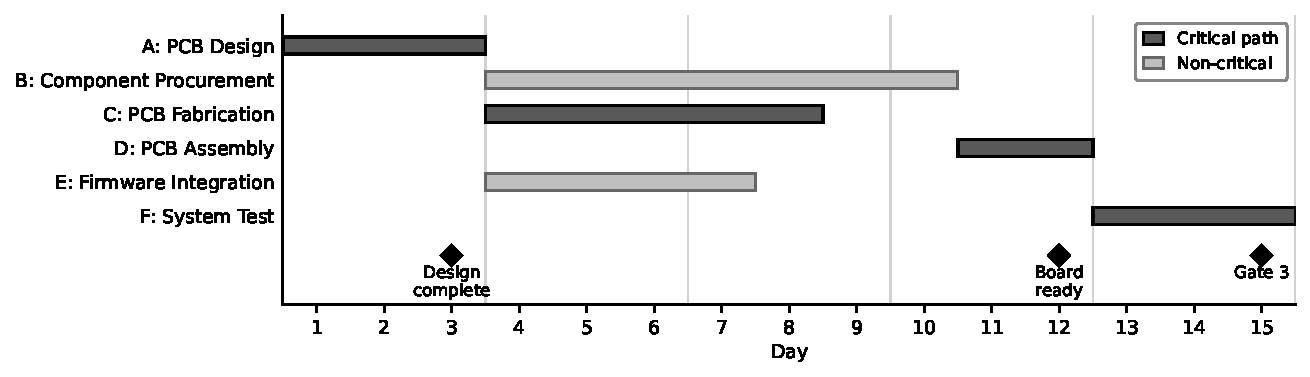
\includegraphics[width=\textwidth]{images/fig_01_gantt}
  \caption{Gantt chart for the sorter prototype build (15~days).
           Solid dark bars are critical-path activities; lighter bars are
           non-critical activities.  The dashed extensions to the right of
           C and E indicate their available slack (2~days and 5~days,
           respectively).  Diamond markers denote milestones.}
  \label{fig:gantt}
\end{figure}

\subsection{Keeping the Gantt alive}

A Gantt chart is not a snapshot taken once at project kickoff; it is a
\textbf{living document}\index{living document} updated at every weekly
check-in.
When Activity~B (component procurement) slips by even one day, the
entire critical path extends by the same amount.
Teams that file the Gantt after sprint planning and never revisit it
are the ones who discover a two-week slip the day before their
gate review.

\paragraph{In Practice.}
Use colour or line-weight to distinguish planned bars from actual
progress bars.  Add a \emph{today} vertical line so any reader can
immediately see what is late.  In a four-person prototype team, a
shared spreadsheet Gantt updated every Monday morning is sufficient;
dedicated project management software adds value only when the WBS
exceeds roughly 20 work packages.

\paragraph{Common Pitfalls.}
When the Gantt is updated but the critical path is not re-evaluated, the team gains false reassurance: the bars move but the slip remains invisible. Any change to a critical-path activity duration must trigger an immediate recalculation of the project end date.

% ============================================================
\section{PERT Three-Point Estimation}
\label{sec:pert}
% ============================================================

CPM uses single-point duration estimates.
For activities with high uncertainty --- particularly procurement ---
that single number conceals the real range of outcomes.
The \textbf{Program Evaluation and Review Technique}
\index{Program Evaluation and Review Technique} (PERT) replaces the
single estimate with three:

\begin{itemize}
  \item $a$ — \textbf{optimistic}\index{optimistic duration}: the
        duration if everything goes well.
  \item $m$ — \textbf{most likely}\index{most likely duration}: the
        mode of the distribution; the single best estimate.
  \item $b$ — \textbf{pessimistic}\index{pessimistic duration}: the
        duration if most things go wrong (short of catastrophe).
\end{itemize}

\subsection{PERT Formulas}

The \textbf{PERT expected duration}\index{PERT!expected duration} is a weighted average placing four times the weight on the most-likely estimate:
\begin{equation}
  t_e = \frac{a + 4m + b}{6}
  \label{eq:ch10-pert-te}
\end{equation}
The \textbf{PERT standard deviation}\index{PERT!standard deviation} quantifies the spread of the estimate:
\begin{equation}
  \sigma = \frac{b - a}{6}
  \label{eq:ch10-pert-sigma}
\end{equation}
A large $\sigma$ warns the team that this activity is a schedule risk even if the expected duration looks acceptable.

\subsection{Worked example: Activity B (component procurement)}

Component procurement is the highest-uncertainty activity on the
critical path.
The team estimates:
\begin{itemize}
  \item $a = 4$~days (supplier has parts in stock, ships next day)
  \item $m = 7$~days (typical online order with standard shipping)
  \item $b = 14$~days (back-order delay or customs hold)
\end{itemize}

Applying Equation~\ref{eq:ch10-pert-te}:
\[
  t_e = \frac{4 + 4(7) + 14}{6}
      = \frac{4 + 28 + 14}{6}
      = \frac{46}{6}
      \approx 7.67\ \text{days}
\]

The CPM single-point estimate of 7~days is slightly optimistic;
the PERT-adjusted estimate of 7.67~days should be used in any
schedule risk analysis.

Applying Equation~\ref{eq:ch10-pert-sigma}:
\[
  \sigma = \frac{14 - 4}{6}
         = \frac{10}{6}
         \approx 1.67\ \text{days}
\]

A standard deviation of 1.67~days on a critical-path activity means
there is a realistic scenario in which the project finishes two or
more days late.
This uncertainty must appear in the risk register (Section~\ref{sec:risk}).

Figure~\ref{fig:pert_dist} illustrates the three-point distribution for
Activity~B with $t_e$ and $\sigma$ annotated.

\begin{figure}[h]
  \centering
  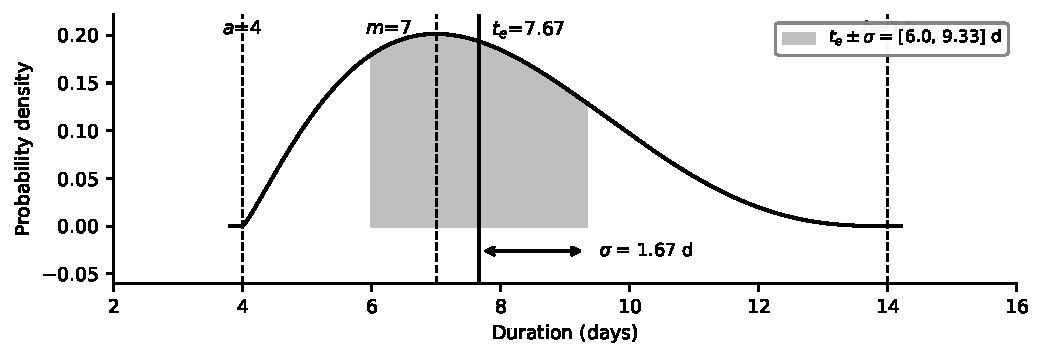
\includegraphics[width=0.7\textwidth]{images/fig_03_pert_dist}
  \caption{PERT distribution for Activity~B (component procurement) with
           $a = 4$~d, $m = 7$~d, $b = 14$~d.
           The expected duration $t_e \approx 7.67$~d is shifted right of
           the mode because the pessimistic tail is longer.
           The $\pm 1\sigma$ band ($\approx 1.67$~d) spans from roughly
           6.0~d to 9.34~d.}
  \label{fig:pert_dist}
\end{figure}

\paragraph{In Practice.}
The asymmetry in the PERT formula ($t_e > m$ when the pessimistic tail
is longer) is intentional and well-founded: in practice, activities
almost always run long rather than short.
When gathering three-point estimates from team members, ask for the
pessimistic estimate last — people systematically underestimate bad
scenarios when they anchor on the most-likely value first.

% ============================================================
\section{Lead Time as a Planning Risk}
\label{sec:leadtime}
% ============================================================

\textbf{Lead time}\index{lead time} is the elapsed calendar time
between placing a component order and having parts in hand.
It is not ``somebody else's problem'' — it is a first-class
\textbf{schedule risk}\index{schedule risk} that must be modelled
explicitly in the network.

\subsection{Why lead time matters on the critical path}

In the sorter schedule, Activity~B (component procurement, $t_e = 7.67$~d)
sits on the critical path.
If the team waits until PCB design is complete before placing an order,
every day of procurement delay directly delays system test.
There is no buffer.

Several mitigation strategies are available:

\begin{enumerate}
  \item \textbf{Preliminary BOM early.}
        Draft a provisional Bill of Materials during detailed design
        (Chapter~11) and place orders before Activity~A is finished.
        This converts B from a strict successor of A into a partial
        overlap, shortening the critical path.
  \item \textbf{Pre-qualify multiple suppliers.}
        If the primary supplier quotes a 14-day lead time, a secondary
        supplier at 7~days keeps the schedule intact.
  \item \textbf{Order buffer stock.}
        For inexpensive passive components (resistors, capacitors)
        the cost of ordering 10\% extra is negligible compared to a
        one-week slip caused by a mis-soldered component that cannot
        be replaced.
  \item \textbf{Expedite only as a last resort.}
        Expediting fees are expensive; build the schedule so that
        expediting is never needed.
\end{enumerate}

\subsection{Long-lead items deserve their own register entries}

Any component with a quoted lead time greater than the slack of its
downstream path belongs in the risk register as its own entry, with a named owner and a specific mitigation plan.
For the sorter, the microcontroller (if on back-order) and the motor
driver IC are the most likely culprits.

\paragraph{Common Pitfalls.}
Teams frequently omit lead time from the schedule entirely, treating
procurement as an instantaneous event.
The result is a day-one crisis: design is ``done'' but parts will not
arrive for ten days and the project duration instantly extends.
Schedule the lead time explicitly, with the same three-point PERT
estimate as any other uncertain activity.

% ============================================================
\section{Maintaining the Risk Register}
\label{sec:risk}
% ============================================================

A \textbf{risk register}\index{risk register} is a living table that
catalogues every identified threat to project objectives, its
likelihood, its impact, and the mitigation strategy the team has
chosen.
It was introduced in Stage~2 with technical risks (Chapter~7).
At Stage~3 it must grow to include \textbf{schedule risks}
\index{schedule risks} and \textbf{procurement risks}
\index{procurement risks}.

\subsection{Standard register fields}

Each row in the register should carry:
\begin{enumerate}
  \item \textbf{ID} — a stable reference code (e.g., R-SCH-01).
  \item \textbf{Description} — one sentence naming the risk event.
  \item \textbf{Likelihood} — Low / Medium / High (or 1–5 scale).
  \item \textbf{Impact} — Low / Medium / High (or 1–5 scale).
  \item \textbf{Risk score} — Likelihood $\times$ Impact.
  \item \textbf{Mitigation} — the specific action the team will take.
  \item \textbf{Owner} — the team member responsible.
  \item \textbf{Status} — Open / In progress / Closed.
\end{enumerate}

\subsection{Schedule-specific risks for the sorter build}

\begin{table}[h]
  \centering
  \caption{Gate~3 risk register entries for the sorter prototype schedule.}
  \label{tab:riskregister}
  \begin{tabular}{p{1.2cm}p{4.5cm}ccp{4.5cm}}
    \hline
    \textbf{ID} & \textbf{Description} &
    \textbf{L} & \textbf{I} & \textbf{Mitigation} \\
    \hline
    R-SCH-01 &
    Component procurement (Act.~B) exceeds 7~days due to supplier
    back-order, delaying system test. &
    M & H &
    Pre-qualify secondary supplier; place order before PCB design
    is finalised. \\[4pt]
    R-SCH-02 &
    PCB fabrication house queue delay extends Act.~C beyond 5~days. &
    L & M &
    Use local fab service with 3-day turnaround as fallback;
    $\geq 2$~days slack available. \\[4pt]
    R-SCH-03 &
    Firmware integration (Act.~E) blocked by undiscovered hardware
    bug discovered at Act.~D, requiring design iteration. &
    M & H &
    Daily smoke-test of assembled PCB before firmware handoff;
    maintain 5~days slack on Act.~E. \\[4pt]
    R-SCH-04 &
    Gate~3 review scheduled on day~14; project duration is 15~days
    — one-day slip causes missed gate. &
    M & H &
    Move gate review to day~16; flag to supervisor immediately if
    Act.~B slips by $>1$~day. \\
    \hline
  \end{tabular}
\end{table}

\subsection{How often to update}

The risk register should be reviewed at every weekly team meeting, in the same session as the Gantt update.
Risks change status: a component that was ``in stock'' last week may
be back-ordered today.
Close a risk only when its triggering condition can no longer occur;
do not close it because the team has stopped worrying about it.

\paragraph{In Practice.}
At Gate~3 reviewers will scan the register for \emph{completeness}
(have schedule and procurement risks been added since Gate~2?) and
\emph{actionability} (do mitigations name a specific person and a
specific action?).
Vague entries such as ``monitor the situation'' are not mitigations;
they are placeholders that signal the team has not thought through
the risk.

% ============================================================
\section*{Try It Yourself}
% ============================================================

\addcontentsline{toc}{section}{Try It Yourself}

The following five-activity network describes a sensor-node firmware
release.

\begin{table}[h]
  \centering
  \caption{Try It Yourself: firmware release work packages.}
  \label{tab:tryit}
  \begin{tabular}{clcl}
    \hline
    \textbf{ID} & \textbf{Work package} & \textbf{Duration (d)} &
    \textbf{Predecessors} \\
    \hline
    P & Requirements review   & 2 & ---  \\
    Q & Driver development    & 6 & P    \\
    R & Unit testing          & 3 & P    \\
    S & Integration testing   & 4 & Q, R \\
    T & Documentation \& release & 2 & S \\
    \hline
  \end{tabular}
\end{table}

\begin{enumerate}
  \item Perform the forward and backward pass to find ES, EF, LS, LF,
        and slack for every activity.
  \item Identify the critical path and state the project duration.
  \item Activity~Q (driver development) has three-point estimates
        $a = 3$~days, $m = 6$~days, $b = 12$~days.
        Use Equations~\ref{eq:ch10-pert-te} and~\ref{eq:ch10-pert-sigma}
        to compute $t_e$ and $\sigma$.
        Substitute $t_e$ for the activity's duration, recompute the total length of each path through the network, and state whether the critical path changes. Show both path lengths explicitly.
  \item Add one schedule risk for this network to a risk register,
        following the format of Table~\ref{tab:riskregister}.
\end{enumerate}

\noindent(No answer key provided.)

% ============================================================
\section*{Review Questions}
% ============================================================

\addcontentsline{toc}{section}{Review Questions}

\begin{enumerate}
  \item \textbf{(Conceptual)} Explain in your own words why the critical
        path is defined by activities with zero slack rather than by the
        activity with the longest duration.
        Give an example where the longest individual activity is
        \emph{not} on the critical path.

  \item \textbf{(Conceptual)} A team builds a Gantt chart on the first
        day of the sprint and does not update it for three weeks.
        Identify two specific ways in which this practice can cause a
        gate failure.

  \item \textbf{(Applied)} A project has four activities:
        W (4~d, no predecessors), X (3~d, predecessor W),
        Y (6~d, predecessor W), Z (2~d, predecessors X and Y).
        Compute ES, EF, LS, LF, and slack for each activity.
        State the critical path and project duration.

  \item \textbf{(Applied)} Activity~Y above has three-point estimates
        $a = 5$~days, $m = 6$~days, $b = 10$~days.
        Compute $t_e$ and $\sigma$ using
        Equations~\ref{eq:ch10-pert-te} and~\ref{eq:ch10-pert-sigma}.
        If the PERT-adjusted duration is used in place of 6~days,
        does the critical path change?  Justify your answer numerically.

  \item \textbf{(Applied --- multi-step)} A project has five activities: J (3~days, no predecessors); K (6~days, predecessor J); L (4~days, predecessor J); M (2~days, predecessors K and L); N (3~days, predecessor M).
  \begin{enumerate}
    \item[(a)] Perform the forward and backward pass. Record ES, EF, LS, LF, and slack for every activity.
    \item[(b)] State the critical path and project duration.
    \item[(c)] Activity~K has three-point estimates $a = 4$~days, $m = 6$~days, $b = 13$~days. Compute $t_e$ and $\sigma$ using Equations~\ref{eq:ch10-pert-te} and~\ref{eq:ch10-pert-sigma}.
    \item[(d)] Write a complete eight-field risk-register entry for the risk that Activity~K exceeds its pessimistic estimate.
  \end{enumerate}
\end{enumerate}

% ============================================================
\section*{End-of-Chapter Artefact}
% ============================================================

\addcontentsline{toc}{section}{End-of-Chapter Artefact}

\textbf{Gate~3 deliverables produced in this chapter:}
\begin{enumerate}
  \item[(a)] \textbf{Gantt chart} — A calendar-based bar chart showing
        all six work packages, their planned start and finish days, the
        critical path highlighted, slack extensions on non-critical
        activities, and milestone markers at days 3, 12, and 15.
        The chart is a living document; it must be updated at every
        team meeting with actual progress.

  \item[(b)] \textbf{Updated risk register} — The Stage~2 technical risk
        register (from Chapter~7) extended with the four schedule and
        procurement risks in Table~\ref{tab:riskregister}.
        Each new entry carries a unique R-SCH-XX identifier, a named
        owner, and a specific — not vague — mitigation action.
        Submit the register as part of the Gate~3 package
        alongside the Gantt chart.
\end{enumerate}

% ============================================================
\section*{Chapter Summary}
% ============================================================

\addcontentsline{toc}{section}{Chapter Summary}

This chapter transformed the sorter team's verified design into a buildable, trackable plan:

\begin{enumerate}
  \item A \textbf{Work Breakdown Structure} decomposed the build into
        six atomic work packages (A through F), each assignable and
        estimable.
  \item The \textbf{CPM forward and backward pass} produced early/late
        start and finish times for every activity.
        Applying Equation~\ref{eq:ch10-slack} revealed that A, B, D,
        and F carry zero slack, making
        \mbox{A\,$\to$\,B\,$\to$\,D\,$\to$\,F} the 15-day critical path.
  \item A \textbf{Gantt chart} (Figure~\ref{fig:gantt}) mapped the
        schedule to a calendar timeline.
        It must be updated weekly; a static Gantt is a liability, not an
        asset.
  \item \textbf{PERT} three-point estimation (Equations
        \ref{eq:ch10-pert-te} and~\ref{eq:ch10-pert-sigma}) quantified
        the uncertainty in Activity~B: $t_e \approx 7.67$~days,
        $\sigma \approx 1.67$~days — a warning that the critical path
        carries real schedule risk.
  \item \textbf{Lead time} is a first-class schedule risk: placing orders
        before PCB design is finalised and pre-qualifying secondary
        suppliers are the primary mitigations.
  \item The \textbf{risk register} was extended with four
        schedule-specific entries (Table~\ref{tab:riskregister}),
        meeting the Gate~3 completeness requirement.
\end{enumerate}

You now have a Gantt chart and an updated risk register — the two
deliverables required for Gate~3 sign-off.
Chapter~11 takes that risk register and the project schedule as its
starting point and builds the full Bill of Materials and procurement
chain, turning the component list implicit in Activity~B into a
concrete sourcing plan with part numbers, quantities, costs, and
supplier alternatives.
